% Options for packages loaded elsewhere
% Options for packages loaded elsewhere
\PassOptionsToPackage{unicode}{hyperref}
\PassOptionsToPackage{hyphens}{url}
%
\documentclass[
  ignorenonframetext,
  aspectratio=169,
  russian,
]{beamer}
\newif\ifbibliography
\usepackage{pgfpages}
\setbeamertemplate{caption}[numbered]
\setbeamertemplate{caption label separator}{: }
\setbeamercolor{caption name}{fg=normal text.fg}
\beamertemplatenavigationsymbolshorizontal
% Prevent slide breaks in the middle of a paragraph
\widowpenalties 1 10000
\raggedbottom
\AtBeginPart{
  \frame{\partpage}
}
\AtBeginSection{
  \ifbibliography
  \else
    \frame{\sectionpage}
  \fi
}
\AtBeginSubsection{
  \frame{\subsectionpage}
}
\usepackage{iftex}
\ifPDFTeX
  \usepackage[T1]{fontenc}
  \usepackage[utf8]{inputenc}
  \usepackage{textcomp} % provide euro and other symbols
\else % if luatex or xetex
  \usepackage{unicode-math} % this also loads fontspec
  \defaultfontfeatures{Scale=MatchLowercase}
  \defaultfontfeatures[\rmfamily]{Ligatures=TeX,Scale=1}
\fi
\usepackage{lmodern}

\ifPDFTeX\else
  % xetex/luatex font selection
\fi
% Use upquote if available, for straight quotes in verbatim environments
\IfFileExists{upquote.sty}{\usepackage{upquote}}{}
\IfFileExists{microtype.sty}{% use microtype if available
  \usepackage[]{microtype}
  \UseMicrotypeSet[protrusion]{basicmath} % disable protrusion for tt fonts
}{}


\usepackage{longtable,booktabs,array}
\usepackage{calc} % for calculating minipage widths
\usepackage{caption}
% Make caption package work with longtable
\makeatletter
\def\fnum@table{\tablename~\thetable}
\makeatother
\usepackage{graphicx}
\makeatletter
\newsavebox\pandoc@box
\newcommand*\pandocbounded[1]{% scales image to fit in text height/width
  \sbox\pandoc@box{#1}%
  \Gscale@div\@tempa{\textheight}{\dimexpr\ht\pandoc@box+\dp\pandoc@box\relax}%
  \Gscale@div\@tempb{\linewidth}{\wd\pandoc@box}%
  \ifdim\@tempb\p@<\@tempa\p@\let\@tempa\@tempb\fi% select the smaller of both
  \ifdim\@tempa\p@<\p@\scalebox{\@tempa}{\usebox\pandoc@box}%
  \else\usebox{\pandoc@box}%
  \fi%
}
% Set default figure placement to htbp
\def\fps@figure{htbp}
\makeatother



\ifLuaTeX
\usepackage[bidi=basic,provide=*]{babel}
\else
\usepackage[bidi=default,provide=*]{babel}
\fi
% get rid of language-specific shorthands (see #6817):
\let\LanguageShortHands\languageshorthands
\def\languageshorthands#1{}


\setlength{\emergencystretch}{3em} % prevent overfull lines

\providecommand{\tightlist}{%
  \setlength{\itemsep}{0pt}\setlength{\parskip}{0pt}}



 

\usepackage[]{csquotes}

\IfFileExists{plex-otf.sty}{
  %% Full TeXlive
   \usepackage[%
     % math,
     RM={Scale=0.94},SS={Scale=0.94},SScon={Scale=0.94},TT={Scale=MatchLowercase,FakeStretch=0.9},DefaultFeatures={Ligatures=Common}
   ]{plex-otf}
}{
  %% TinyTeX
  \usepackage{libertine}
}

%%% Load theme
% https://deic.uab.cat/~iblanes/beamer_gallery/
\IfFileExists{beamerthemegotham.sty}{
  %% Full TeXlive
  \usetheme{gotham}
  \gothamset{
    numbering=totalpagenumber,
    parttocframe default=off,
    sectiontocframe default=off,
    subsectiontocframe default=off,
  }
}{
  %% TinyTeX
  \usetheme{Madrid}
}
\makeatletter
\@ifpackageloaded{caption}{}{\usepackage{caption}}
\AtBeginDocument{%
\ifdefined\contentsname
  \renewcommand*\contentsname{Содержание}
\else
  \newcommand\contentsname{Содержание}
\fi
\ifdefined\listfigurename
  \renewcommand*\listfigurename{Список иллюстраций}
\else
  \newcommand\listfigurename{Список иллюстраций}
\fi
\ifdefined\listtablename
  \renewcommand*\listtablename{Список таблиц}
\else
  \newcommand\listtablename{Список таблиц}
\fi
\ifdefined\figurename
  \renewcommand*\figurename{Рисунок}
\else
  \newcommand\figurename{Рисунок}
\fi
\ifdefined\tablename
  \renewcommand*\tablename{Таблица}
\else
  \newcommand\tablename{Таблица}
\fi
}
\@ifpackageloaded{float}{}{\usepackage{float}}
\floatstyle{ruled}
\@ifundefined{c@chapter}{\newfloat{codelisting}{h}{lop}}{\newfloat{codelisting}{h}{lop}[chapter]}
\floatname{codelisting}{Список}
\newcommand*\listoflistings{\listof{codelisting}{Листинги}}
\makeatother
\makeatletter
\makeatother
\makeatletter
\@ifpackageloaded{caption}{}{\usepackage{caption}}
\@ifpackageloaded{subcaption}{}{\usepackage{subcaption}}
\makeatother

\usepackage{bookmark}
\IfFileExists{xurl.sty}{\usepackage{xurl}}{} % add URL line breaks if available
\urlstyle{same}
\hypersetup{
  pdftitle={Цели и задачи защиты информации. Организация защиты конфиденциальной информации},
  pdfauthor={Трусова Алина Александровна},
  pdflang={ru-RU},
  hidelinks,
  pdfcreator={LaTeX via pandoc}}


\title{Цели и задачи защиты информации. Организация защиты
конфиденциальной информации}
\subtitle{Основы информационной безопасности}
\author{Трусова Алина Александровна}
\date{2026-04-03}

\begin{document}
\frame{\titlepage}

\renewcommand*\contentsname{Содержание}
\begin{frame}[allowframebreaks]
  \frametitle{Содержание}
  \setcounter{tocdepth}{2}
  \tableofcontents
\end{frame}
\setcounter{tocdepth}{2}
\tableofcontents
}

\section{1. Информация}\label{ux438ux43dux444ux43eux440ux43cux430ux446ux438ux44f}

\begin{frame}{1.1 Докладчик}
\phantomsection\label{ux434ux43eux43aux43bux430ux434ux447ux438ux43a}
\begin{columns}[c]
\begin{column}{0.7\linewidth}
\begin{itemize}[<+->]
\tightlist
\item
  Трусова Алина Александровна
\item
  Студент
\item
  Российский университет дружбы народов им. П. Лумумбы
\item
  \href{mailto:1132246715@rudn.ru}{\nolinkurl{1132246715@rudn.ru}}
\item
  \url{https://alas-aline.github.io/}
\end{itemize}
\end{column}

\begin{column}{0.3\linewidth}
\pandocbounded{
\includegraphics[keepaspectratio]{./image/me.png}}
\end{column}
\end{columns}
\end{frame}

\section{2. Вводная
часть}\label{ux432ux432ux43eux434ux43dux430ux44f-ux447ux430ux441ux442ux44c}

\begin{frame}{2.1 Актуальность}
\phantomsection\label{ux430ux43aux442ux443ux430ux43bux44cux43dux43eux441ux442ux44c}
\begin{itemize}[<+->]
\tightlist
\item
  Информационные активы ---- ключевой ресурс
\item
  Новые схемы мошенничества
\item
  Недостаточная осведомлённость
\item
  Растёт количество случаев кражи данных
\end{itemize}
\end{frame}

\begin{frame}{2.2 Объект и предмет исследования}
\phantomsection\label{ux43eux431ux44aux435ux43aux442-ux438-ux43fux440ux435ux434ux43cux435ux442-ux438ux441ux441ux43bux435ux434ux43eux432ux430ux43dux438ux44f}
\begin{itemize}[<+->]
\tightlist
\item
  Информационная безопасность
\item
  Криптография
\item
  Входные и выходные форматы презентаций
\end{itemize}
\end{frame}

\begin{frame}{2.3 Цели и задачи}
\phantomsection\label{ux446ux435ux43bux438-ux438-ux437ux430ux434ux430ux447ux438}
\begin{itemize}[<+->]
\tightlist
\item
  Повысить осведомлённость об информационной безопасности
\item
  Узнать о способах защиты информации
\end{itemize}
\end{frame}

\section{3. Понятие информационной
безопасности}\label{ux43fux43eux43dux44fux442ux438ux435-ux438ux43dux444ux43eux440ux43cux430ux446ux438ux43eux43dux43dux43eux439-ux431ux435ux437ux43eux43fux430ux441ux43dux43eux441ux442ux438}

\begin{frame}{3.1 Что такое информационная безопасность?}
\phantomsection\label{ux447ux442ux43e-ux442ux430ux43aux43eux435-ux438ux43dux444ux43eux440ux43cux430ux446ux438ux43eux43dux43dux430ux44f-ux431ux435ux437ux43eux43fux430ux441ux43dux43eux441ux442ux44c}
Определение:

\begin{itemize}[<+->]
\tightlist
\item
  Состояние защищенности информации и поддерживающей инфраструктуры
\item
  Защита от случайных или преднамеренных воздействий
\item
  Обеспечение нормального функционирования объекта
\end{itemize}

Нормативная база (РФ):

\begin{itemize}[<+->]
\tightlist
\item
  Доктрина информационной безопасности РФ
\item
  ГОСТ Р 50922-2006
\end{itemize}
\end{frame}

\begin{frame}{3.2 Базовые цели защиты информации (CIA Triad)}
\phantomsection\label{ux431ux430ux437ux43eux432ux44bux435-ux446ux435ux43bux438-ux437ux430ux449ux438ux442ux44b-ux438ux43dux444ux43eux440ux43cux430ux446ux438ux438-cia-triad}
\pandocbounded{\includegraphics[keepaspectratio]{infosec--lab03--presentation_files/mediabag/83a0732c2407bb16da3d.png}}
\end{frame}

\begin{frame}[fragile]{3.3 Задачи системы защиты информации}
\phantomsection\label{ux437ux430ux434ux430ux447ux438-ux441ux438ux441ux442ux435ux43cux44b-ux437ux430ux449ux438ux442ux44b-ux438ux43dux444ux43eux440ux43cux430ux446ux438ux438}
\begin{columns}[c]
\begin{column}{0.7\linewidth}
\begin{verbatim}
Список задач:

- Предотвращение утечек и несанкционированного доступа
- Своевременное обнаружение инцидентов (мониторинг)
- Минимизация последствий атак (восстановление)
- Правовое регулирование отношений в области ИБ
- Обучение персонала культуре безопасности
\end{verbatim}
\end{column}

\begin{column}{0.3\linewidth}
\pandocbounded{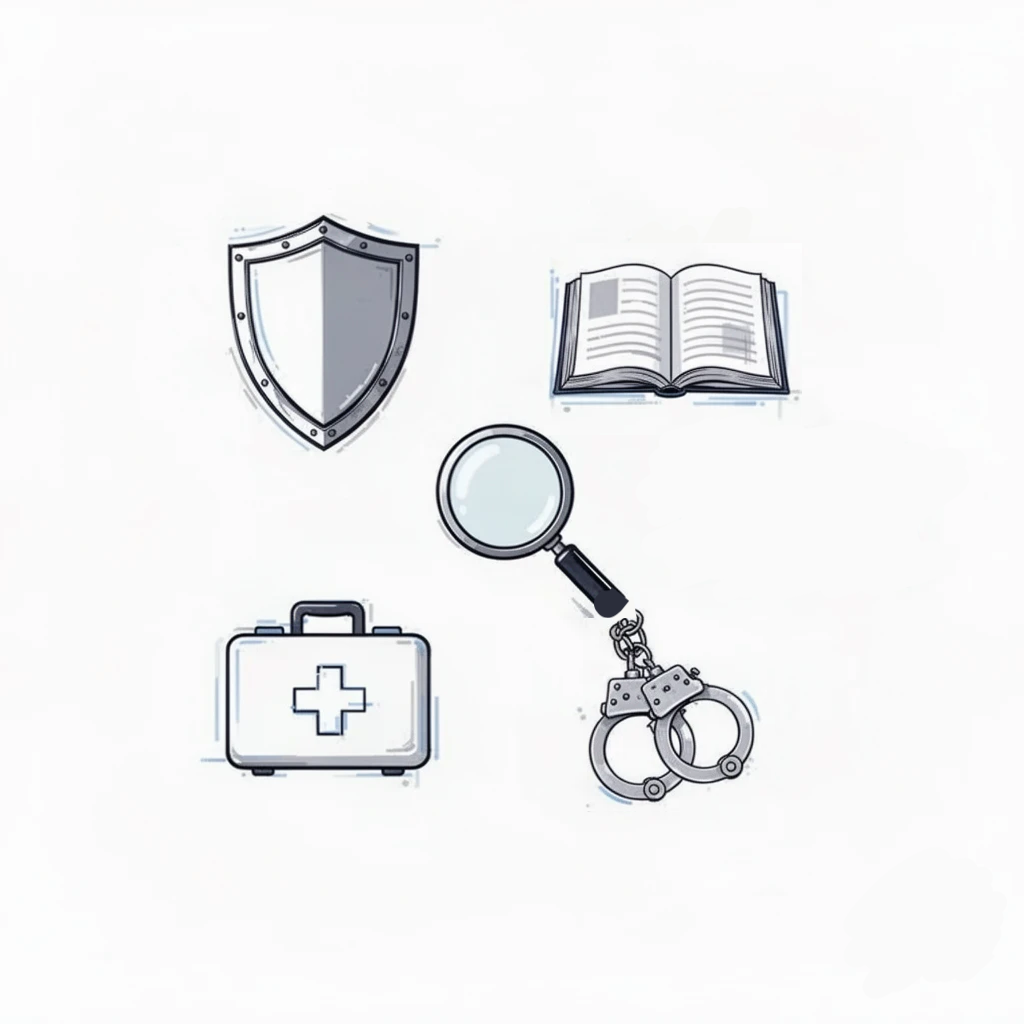
\includegraphics[keepaspectratio]{./image/1.png}}
\end{column}
\end{columns}
\end{frame}

\begin{frame}{3.4 Конфиденциальная информация: виды}
\phantomsection\label{ux43aux43eux43dux444ux438ux434ux435ux43dux446ux438ux430ux43bux44cux43dux430ux44f-ux438ux43dux444ux43eux440ux43cux430ux446ux438ux44f-ux432ux438ux434ux44b}
\pandocbounded{\includegraphics[keepaspectratio]{infosec--lab03--presentation_files/mediabag/wzym6p2fkflph756rhk2.png}}
\end{frame}

\section{4. Система защиты конфиденциальной информации
(СЗКИ)}\label{ux441ux438ux441ux442ux435ux43cux430-ux437ux430ux449ux438ux442ux44b-ux43aux43eux43dux444ux438ux434ux435ux43dux446ux438ux430ux43bux44cux43dux43eux439-ux438ux43dux444ux43eux440ux43cux430ux446ux438ux438-ux441ux437ux43aux438}

\begin{frame}{4.1 Принципы построения:}
\phantomsection\label{ux43fux440ux438ux43dux446ux438ux43fux44b-ux43fux43eux441ux442ux440ux43eux435ux43dux438ux44f}
\begin{itemize}[<+->]
\tightlist
\item
  Комплексность (сочетание мер)
\item
  Непрерывность процесса
\item
  Своевременность внедрения
\item
  Разумная достаточность (баланс затрат и рисков)
\end{itemize}
\end{frame}

\begin{frame}{4.2 Этапы:}
\phantomsection\label{ux44dux442ux430ux43fux44b}
\pandocbounded{
\includegraphics[keepaspectratio]{infosec--lab03--presentation_files/mediabag/The-PDCA-Cycle-01-2.png}}
\end{frame}

\begin{frame}{4.3 Организационные меры защиты}
\phantomsection\label{ux43eux440ux433ux430ux43dux438ux437ux430ux446ux438ux43eux43dux43dux44bux435-ux43cux435ux440ux44b-ux437ux430ux449ux438ux442ux44b}
Инструменты:

\begin{itemize}[<+->]
\tightlist
\item
  Разработка нормативных документов (Политики, Инструкции)
\item
  Режим пропускного контроля (физическая защита)
\item
  Работа с персоналом (NDA, подписка о неразглашении)
\item
  Управление доступом (принцип минимальных привилегий)
\item
  Учет и маркировка носителей информации
\end{itemize}
\end{frame}

\begin{frame}{4.4 Технические средства защиты}
\phantomsection\label{ux442ux435ux445ux43dux438ux447ux435ux441ux43aux438ux435-ux441ux440ux435ux434ux441ux442ux432ux430-ux437ux430ux449ux438ux442ux44b}
\begin{itemize}[<+->]
\tightlist
\item
  Средства идентификации и аутентификации: Пароли, токены, биометрия
\item
  Средства разграничения доступа: СЗИ от НСД
\item
  Средства криптографии: Шифрование каналов и данных (ЭЦП, VPN)
\item
  Межсетевые экраны и антивирусы: Защита периметра
\item
  DLP-системы: Предотвращение утечек данных
\end{itemize}
\end{frame}

\section{5. Правовое регулирование в
РФ}\label{ux43fux440ux430ux432ux43eux432ux43eux435-ux440ux435ux433ux443ux43bux438ux440ux43eux432ux430ux43dux438ux435-ux432-ux440ux444}

\begin{frame}{5.1 Нормативно-правовая база (РФ)}
\phantomsection\label{ux43dux43eux440ux43cux430ux442ux438ux432ux43dux43e-ux43fux440ux430ux432ux43eux432ux430ux44f-ux431ux430ux437ux430-ux440ux444}
Ключевые законы:

\begin{itemize}[<+->]
\tightlist
\item
  ФЗ №149: «Об информации, информационных технологиях и о защите
  информации»
\item
  ФЗ №152: «О персональных данных»
\item
  ФЗ №98: «О коммерческой тайне»
\item
  ФЗ №187: «О безопасности критической информационной инфраструктуры»
\item
  Указы Президента и приказы ФСТЭК/ФСБ
\end{itemize}
\end{frame}

\section{6. Выводы}\label{ux432ux44bux432ux43eux434ux44b}

\begin{frame}{6. Выводы}
\pandocbounded{\includegraphics[keepaspectratio]{infosec--lab03--presentation_files/mediabag/-Удобство-}}
\end{frame}




\end{document}
